%----------------------------------------------------------------------------------------
%	PACKAGES AND OTHER DOCUMENT CONFIGURATIONS
%----------------------------------------------------------------------------------------

\documentclass[twoside,twocolumn,a4paper]{article}

\usepackage{blindtext} % Package to generate dummy text throughout this template 

\usepackage{mhchem}

\usepackage[T1]{fontenc} % Use 8-bit encoding that has 256 glyphs

\usepackage{lmodern}

\usepackage[hyphenbreaks]{breakurl}

\usepackage[hyphens]{url}

%\usepackage[super,sort&compress]{natbib}
%\usepackage{natbib}
%\setlength{\bibsep}{0.0pt}

\usepackage{graphicx}

\linespread{1.05} % Line spacing - Palatino needs more space between lines
\usepackage{microtype} % Slightly tweak font spacing for aesthetics

\usepackage[spanish]{babel} % Language hyphenation and typographical rules

\usepackage[numbib,notlof,notlot,nottoc]{tocbibind} % Shows bibliography as a section

\usepackage[hmarginratio=1:1,top=32mm,columnsep=20pt]{geometry} % Document margins

\usepackage[hang, small,labelfont=bf,up,textfont=up]{caption} % Custom captions under/above floats in tables or figures

\usepackage[section]{placeins}

\usepackage{float}

\usepackage{booktabs} % Horizontal rules in tables

\usepackage{enumitem} % Customized lists

\setlist[itemize]{noitemsep} % Make itemize lists more compact

\usepackage{abstract} % Allows abstract customization

\renewcommand{\abstractnamefont}{\normalfont\bfseries} % Set the "Abstract" text to bold

\usepackage{fancyhdr} % Headers and footers
\pagestyle{fancy} % All pages have headers and footers
\fancyhead{} % Blank out the default header
\fancyfoot{} % Blank out the default footer
\fancyhead[C]{Laboratorio 4 $\bullet$ Informe 2 $\bullet$ Grupo 3: Poggi, R\'ios Ch\'avez} % Custom header text
\fancyfoot[C]{\thepage} % Custom footer text

\usepackage{titling} % Customizing the title section

\usepackage{hyperref} % For hyperlinks in the PDF

%----------------------------------------------------------------------------------------
%	TITLE SECTION
%----------------------------------------------------------------------------------------

\setlength{\droptitle}{-4\baselineskip} % Move the title up

\pretitle{\begin{center}\LARGE\bfseries} % Article title formatting
\posttitle{\end{center}} % Article title closing formatting
\title{Difusividad t\'ermica} % Article title
\author{%
\textsc{Ignacio Poggi} \\[1ex] % Your name
\normalsize \href{mailto:ignaciop.3@gmail.com}{ignaciop.3@gmail.com} % Your email address
\and % Uncomment if 2 authors are required, duplicate these 4 lines if more
\textsc{Carlos R\'ios Ch\'avez} \\[1ex] % Second author's name
\normalsize \href{mailto:carlos_rios_ch@hotmail.com}{carlos\_rios\_ch@hotmail.com} % Second author's email address
}



\date{Grupo 3 - Laboratorio 4, C\'atedra Schmiegelow - Departamento de F\'isica, Facultad de Ciencias Exactas y Naturales, Universidad de Buenos Aires \newline \\ \today} % Leave empty to omit a date
\renewcommand{\maketitlehookd}{%
\begin{abstract}
\noindent En este trabajo se estudi\'o la  difusi\'on  del  calor utilizando una barra de cobre sometida a una fuente peri\'odica, modulada por una onda cuadrada en uno de sus extremos. Se calcul\'o la velocidad y el coeficiente de decaimiento de la onda de calor en el estado estacionario, para poder obtener la constante de difusividad t\'ermica del \ce{_{29}Cu}, $\kappa = ALGO$.

\end{abstract}
}

%----------------------------------------------------------------------------------------

\begin{document}
\maketitle

% Print the title

%----------------------------------------------------------------------------------------
%	ARTICLE CONTENTS
%----------------------------------------------------------------------------------------

\section{Introducci\'on}

En un s\'olido is\'otropo y homog\'eneo, cuya difusividad t\'ermica $\kappa$ es independiente de la temperatura, la ecuaci\'on que determina el comportamiento t\'ermico es: \cite{eq:calor}:

\begin{equation}
\label{eq:calor}
\frac{\partial^2 \theta (x,t)}{\partial x^{2}} = \frac{1}{\kappa} \frac{\partial \theta (x,t)}{\partial t}
\end{equation}

siendo $\theta(x,t)$ la temperatura en la posici\'on $x$ a tiempo $t$. A la ecuaci\'on (\ref{eq:calor}) se la conoce como la ecuaci\'on de Fourier unidimensional. Para determinar las condiciones de contorno que corresponden a nuestro experimento, se dispuso en el origen de la barra una fuente de calor peri\'odica, lo que permite expresar $\theta(x,t)$ en este extremo de la siguiente manera:

\begin{equation}
\label{eq:theta0}
\theta(0,t) = \sum_{n = 1, 3, 5, ...}^{\infty} \frac{4\theta_{0}}{n\pi} sen(\frac{2n\pi t}{\tau})
\end{equation}

Adem\'as, como la barra se supone semi-infinita, la condici\'on en el otro extremo ser\'a $\theta(\infty,t) = 0$; es decir, se considera que la temperatura al final de la barra decae completamente. \newline

\par
Siendo que nos interesa la distribuci\'on de temperatura en el r\'egimen estacionario, se propone la siguiente serie de Fourier como soluci\'on a la ecuaci\'on (\ref{eq:calor}):

\begin{equation}
\label{eq:solgeneral}
\theta(x,t) = \sum_{n = 1}^{\infty} A_{n}(x) sen(\omega_{n}t - k_{n}x)
\end{equation}

donde $A_{n}$, $\omega_{n}$ y $k_{n}$ son la amplitud, frecuencia y el n\'umero de onda del $n$-\'esimo arm\'onico. Reemplazando la ecuaci\'on (\ref{eq:solgeneral}) en (\ref{eq:calor}), junto a las condiciones de contorno mencionadas en (\ref{eq:theta0}) y $\theta(\infty,t) = 0$, se obtiene la soluci\'on para el sistema estudiado:

\begin{equation}
\label{eq:solbarra}
\theta(x,t) = \sum_{n = 1, 3, 5, ...}^{\infty} \theta_{n}e^{\epsilon_{n}x} sen(\omega_{n}t - \epsilon_{n}x)
\end{equation}

donde

\begin{equation}
\label{eq:conds}
\theta_{n} = \frac{4\theta_{0}}{n\pi}, \omega_{n} = \frac{2n\pi t}{\tau}, \epsilon_{n} = \sqrt{\frac{\omega_{n}}{2\kappa}}
\end{equation}


Se puede ver que, a medida que aumenta $n$, los arm\'onicos se desvanecen r\'apidamente dado que $\epsilon_{n}$ aumenta con la frecuencia. Debido a esto, es posible aproximar a la distribuci\'on de temperatura en puntos lo suficientemente alejados del origen de la barra, utilizando solamente el primer arm\'onico:

\begin{equation}
\label{eq:firstharmonic}
\theta(x,t) \approx A_{0}e^{\epsilon x} cos(\omega(t - \frac{x}{v}))
\end{equation}

escogiendo el origen de tiempo tal que $\theta$ es m\'aximo en $ x = 0$. Considerando la ecuaci\'on (\ref{eq:firstharmonic}) y el primer arm\'onico de la soluci\'on completa (\ref{eq:solbarra}), se pueden obtener las expresiones:

\begin{equation}
\label{eq:ke}
\kappa_{\epsilon} = \frac{pi}{\tau \epsilon^{2}}
\end{equation}

\begin{equation}
\label{eq:kv}
\kappa_{v} = \frac{v^{2} \tau}{4\pi}
\end{equation}


que relacionan las propiedades t\'ermicas del material, en este caso la difusividad t\'ermica $\kappa$, con dos propiedades de la onda: la velocidad $v$ y el coeficiente de decaimiento $\epsilon$. \newline

\par
Finalmente, combinando las ecuaciones (\ref{eq:ke}) y (\ref{eq:kv}), se obtiene una expresi\'on para el coeficiente de difusividad t\'ermica en funci\'on de los par\'ametros $v$ y $\epsilon$, determinados experimentalmente:

\begin{equation}
\label{eq:kappa}
\kappa = \frac{v}{2\epsilon}
\end{equation}

%------------------------------------------------

\section{Dispositivo experimental}

Los instrumentos de laboratorio utilizados en ambos m\'etodos fueron:
\begin{itemize}
\item 
\label{Laser} L\'aser marca Melles Griot, modelo 06DAL003 de 670 nm.
\item Espejos marca Melles Griot.
\item Pesos y soporte para pesos.
\item Barras de lat\'on y de hierro de diferentes longitudes y pesos.
\item Rendija de metal.
\item Fotodiodo marca ThorLabs, modelo DET36A/M.
\item Placa de adquisici\'on de datos marca National Instruments, modelo NIUSB-6212.
\item Computadora personal con software MATLAB para la recolecci\'on y an\'alisis de datos.
\end{itemize}

\subsection{M\'etodo est\'atico}

En el armado experimental (Figura \ref{fig:disenoestatico}) de este m\'etodo se utilizaron dos cuchillas que nos sirvieron para armar la rendija por la cual se producir\'ia la difracci\'on. Se fij\'o una de las cuchillas al extremo libre de la varilla de lat\'on (el di\'ametro de la varilla es de $d = 0.470 \pm 0.002cm$) y se fij\'o la otra cuchilla en un punto m\'as alto que la primera. De \'esta manera, al colocar diferentes pesos al extremo libre de la varilla, \'esta se deform\'o produciendo diferentes patrones de difracci\'on. Las masas utilizadas fueron las siguientes: $m_{1} = 22,57 g$, $m_{2} = 26,22 g$, $m_{3} = 20,66 g$, $m_{4} = 27,85 g$, $m_{5} = 28,48 g$, $m_{6} = 18,75 g$, $m_{7} = 12,66 g$, $m_{8} = 22,40 g$, cabe considerar que en estos valores est\'a incluida la masa del soporte utilizado, y por otro lado que las mediciones se efectuaron con una balanza de alta precisi\'on marca Ohaus Analytical Plus , modelo AP210, que tiene un error del \'orden de los miligramos y que por lo tanto no lo consideramos. \newline

\begin{figure}[H]
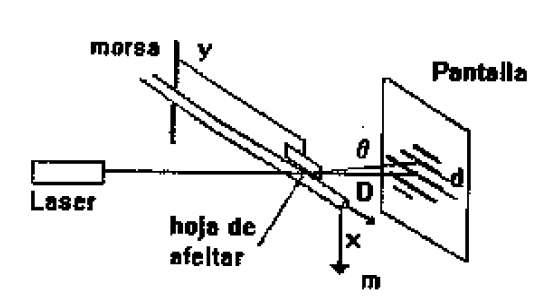
\includegraphics[width=\linewidth]{disenoestatico.png}
\caption{Disposici\'on experimental del m\'etodo est\'atico.}
\label{fig:disenoestatico}
\end{figure}

Se utiliz\'o un l\'aser con una longitud de onda $\lambda= 670 nm$ (color rojo). Para que el haz del l\'aser impactara justo en la rendija se utiliz\'o un arreglo de espejos. De esta manera, se tom\'o registro en un papel de los patrones de difracci\'on generados a una distancia $D = 155,1 \pm 0,1 cm$ de la rendija; en la Figura \ref{fig:difrac} se puede ver un ejemplo de uno de los patrones de difracci\'on observados. Posteriormente, se midi\'o con una regla las distancias entre los m\'aximos registrados en el papel, se realizaron ocho mediciones con distintos pesos.

\begin{figure}[H]
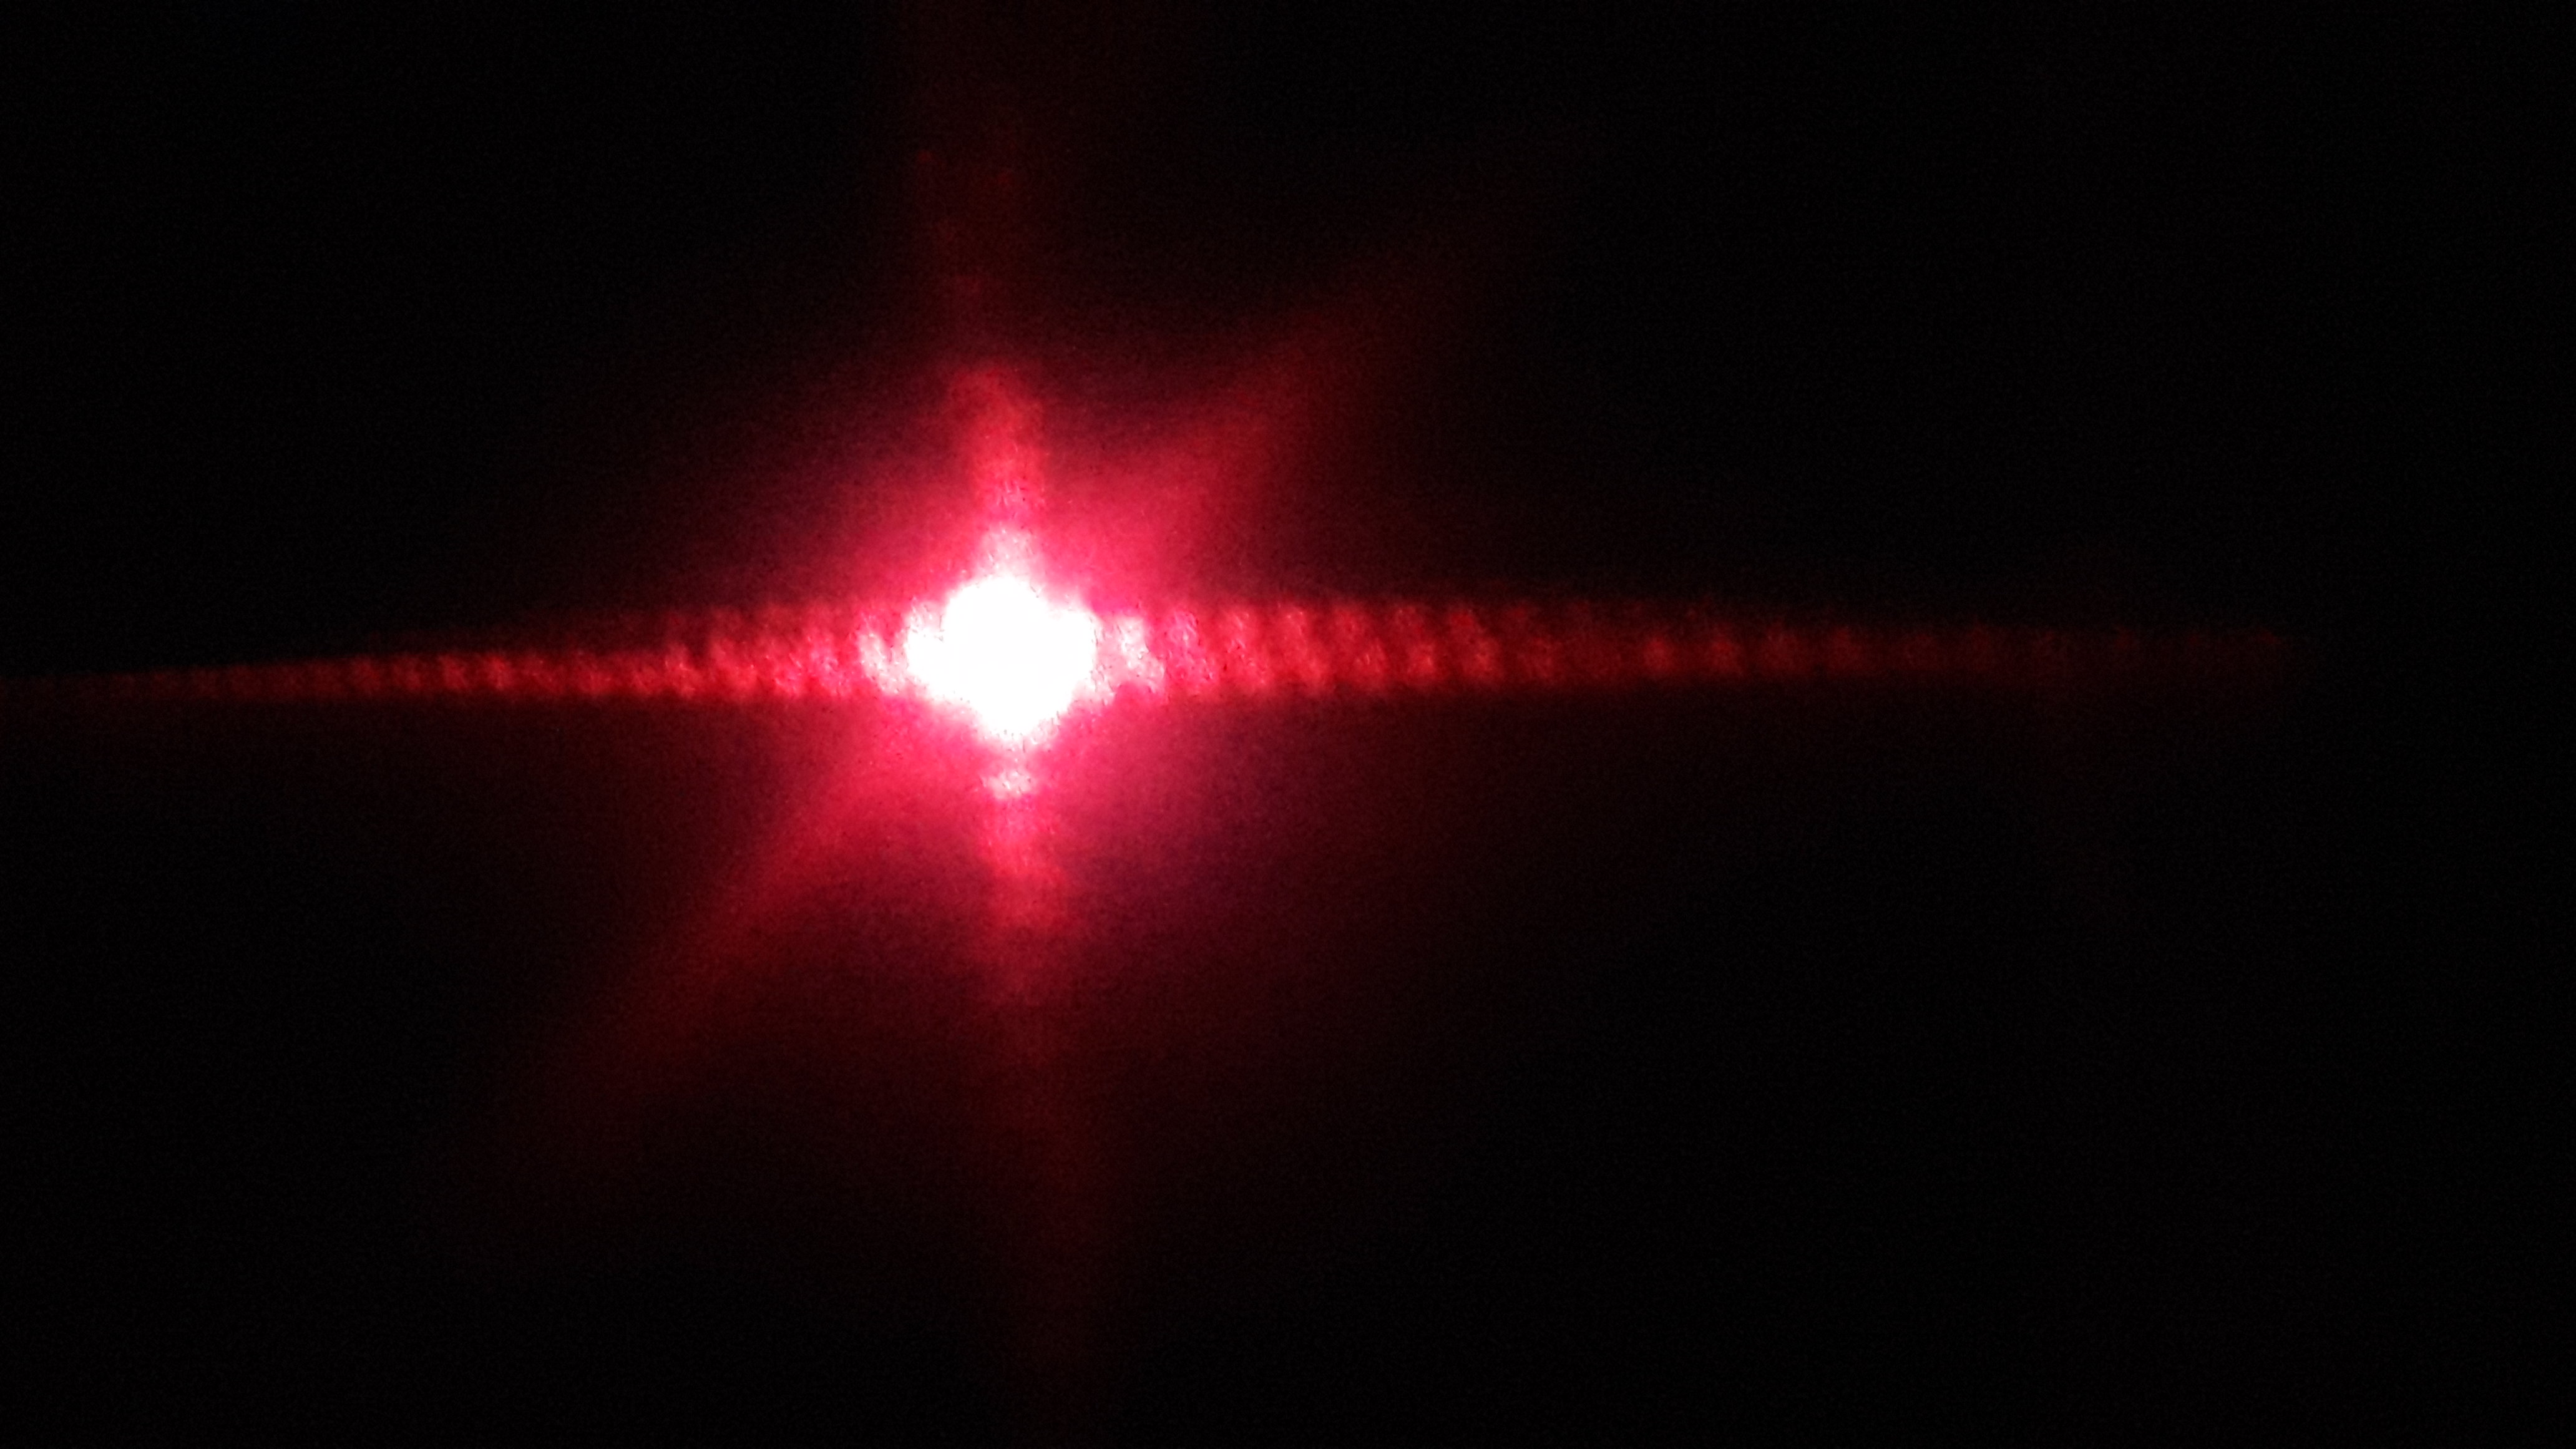
\includegraphics[width=\linewidth]{difrac.jpg}
\caption{Ejemplo del fen\'omeno de difracci\'on observado en el experimento.}
\label{fig:difrac}
\end{figure}

\subsection{M\'etodo din\'amico}

Para este m\'etodo se utiliz\'o pr\'acticamente el mismo dispositivo experimental que en el est\'atico, con la excepci\'on de que se quitaron los pesos y se utilizaron dos barras de lat\'on (diferenciandose entre s\'i por su di\'ametro, longitud y peso) y otra de hierro. En la siguiente tabla se detallan los valores tomados para cada barra:\newline

\begin{table}[H]
\centering
\caption{Di\'ametros $d$, longitudes $L$ y pesos $m$ de las tres barras utilizadas.}
\label{tab:valoresbarras}
\begin{tabular}{|c|c|c|c|}
\hline
Material & $d$ $\pm$ 0,002 & $L$ $\pm$ 0,1 & $m$ $\pm$ 0,1\\ \hline
Lat\'on & 0,471 cm & 31,02 cm & 51,22 g\\ \hline
Hierro & 0,369 cm & 36,10 cm & 36,57 g  \\ \hline
Lat\'on fino & 0,243 cm & 40,30 cm & 22,02 g \\ \hline
\end{tabular}
\end{table}


Adem\'as, se agreg\'o un fotodiodo de \ce{^{28}_{14}Si} marca ThorLabs modelo DET36A/M justo detr\'as del extremo libre de la barra para poder registrar las oscilaciones verticales de la misma. \newline
\'Este \'ultimo se conect\'o a una placa de adquisici\'on de datos marca National Instruments NIUSB-6212, y mediante un programa hecho en MATLAB se registr\'o, durante 60 segundos y a una frecuencia de 1000 Hz, la se\~nal capturada por el fotodiodo. En la Figura (\ref{fig:dispexp_dinamico}) se muestra este arreglo experimental.

\begin{figure}[H]
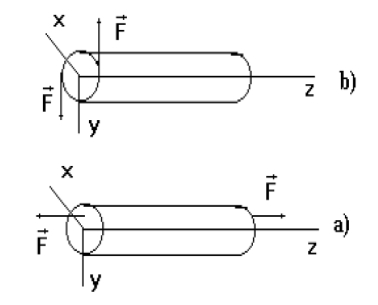
\includegraphics[width=\linewidth]{momentos.jpg}
\caption{Dispositivo experimental utilizado en el m\'etodo din\'amico. Se pueden ver los siguientes elementos: A) L\'aser, B) Barra y soporte, C) Espejos para redireccionar el haz hacia el extremo libre de la barra, D) Fotodiodo.}
\label{fig:dispexp_dinamico}
\end{figure}

Cabe destacar que, para poder estar seguros de que la frecuencia de 1000 Hz elegida para el sampleo de los datos era suficiente; se realiz\'o un breve c\'alculo a mano para obtener las frecuencias de oscilaci\'on de los tres primeros modos mediante las ecuaciones (\ref{eq:omegas}) y (\ref{eq:condiciones}), tomando $\alpha = 0$; dando como resultado valores de $f_{k} < 500$ Hz, con lo cual se satisfacieron las condiciones del teorema de Nyquist-Shannon \cite{teo:shannon}

La determinaci\'on del factor de amortiguamiento $\alpha$ se llevo a cabo mediante un ajuste sobre la se\~nal original con una forma funcional senoidal amortiguada exponencialmente.
Para calcular las frecuencias $f_{k}$, se realiz\'o un an\'alisis de Fourier sobre la se\~nal obtenida por el fotodiodo y as\'i poder obtener el valor del m\'odulo de Young $E$ mediante la ecuaci\'on (\ref{eq:omegas}) y la constante de amortiguamiento previamente calculada.

Por \'ultimo, para la barra de lat\'on fino se analiz\'o como varia la frecuencia fundamental y el factor de amortiguamiento en funci\'on de la longitud de la barra (cambiando la posici\'on del extremo fijo de la misma), partiendo de $L_{1} = 40,3 \pm 0,1$ cm, en decrementos de 4 cm, hasta $L_{6} = 20,3 \pm 0,1$ cm.



%------------------------------------------------
\section{Resultados y an\'alisis}

\subsection{M\'etodo est\'atico}

Para conocer la deformaci\'on de la varilla de lat\'on mediante el fen\'omeno de difracci\'on se utiliz\'o la ecuaci\'on \ref{eq:minimos} que sale de las ecuaciones que describen los m\'inimos de la  difracci\'on de  Fraunhofer, donde $\lambda$  es la longitud de onda, $D$ es la distancia de la rendija a la pantalla, $n$ es el n\'umero de m\'inimo ($n = 1, 2, 3...$), $d_{n}$ es la distancia a la cual se encuentra dicho m\'inimo, y la variable $y$ representa la apertura de la rendija, o en otros t\'erminos, representa la deformaci\'on de la varilla.

\begin{equation}
\label{eq:minimos}
y= \lambda D \frac{n}{d_{n}}
\end{equation}

Considerando que en la toma de datos los m\'aximos de intensidad son mucho m\'as definidos que los m\'inimos, se midieron las posiciones de los m\'aximos. Sin embargo en la ecuaci\'on \ref{eq:minimos} se precisan las posiciones de los puntos donde la intensidad es m\'inima. Para obtener estos m\'inimos se calcularon los puntos medios entre dos m\'aximos. Entonces, mediante la ecuaci\'on \ref{eq:minimos} se obtuvo una lista, por cada patr\'on de difracci\'on, que conten\'ia varios valores de $y$ (el ancho de la rejilla). Se promediaron dichos valores y considerando que cada promedio correspond\'ia a un peso distinto se realiz\'o una regresi\'on lineal entre los valores de masa-deformaci\'on, en la cual se obtuvo una pendiente de $-0,00285 \pm 0,00014 $ y una abscisa de $0,147 \pm 0,006$ (Figura \ref{fig:regrlin}). Comparando este resultado con nuestro modelo te\'orico expresado en la ecuaci\'on \ref{eq:vigafeynman} , se obtuvo un m\'odulo de Young de $E = (16,28 \pm 3,87) * 10^{10} Pa$.

\begin{figure}[H]
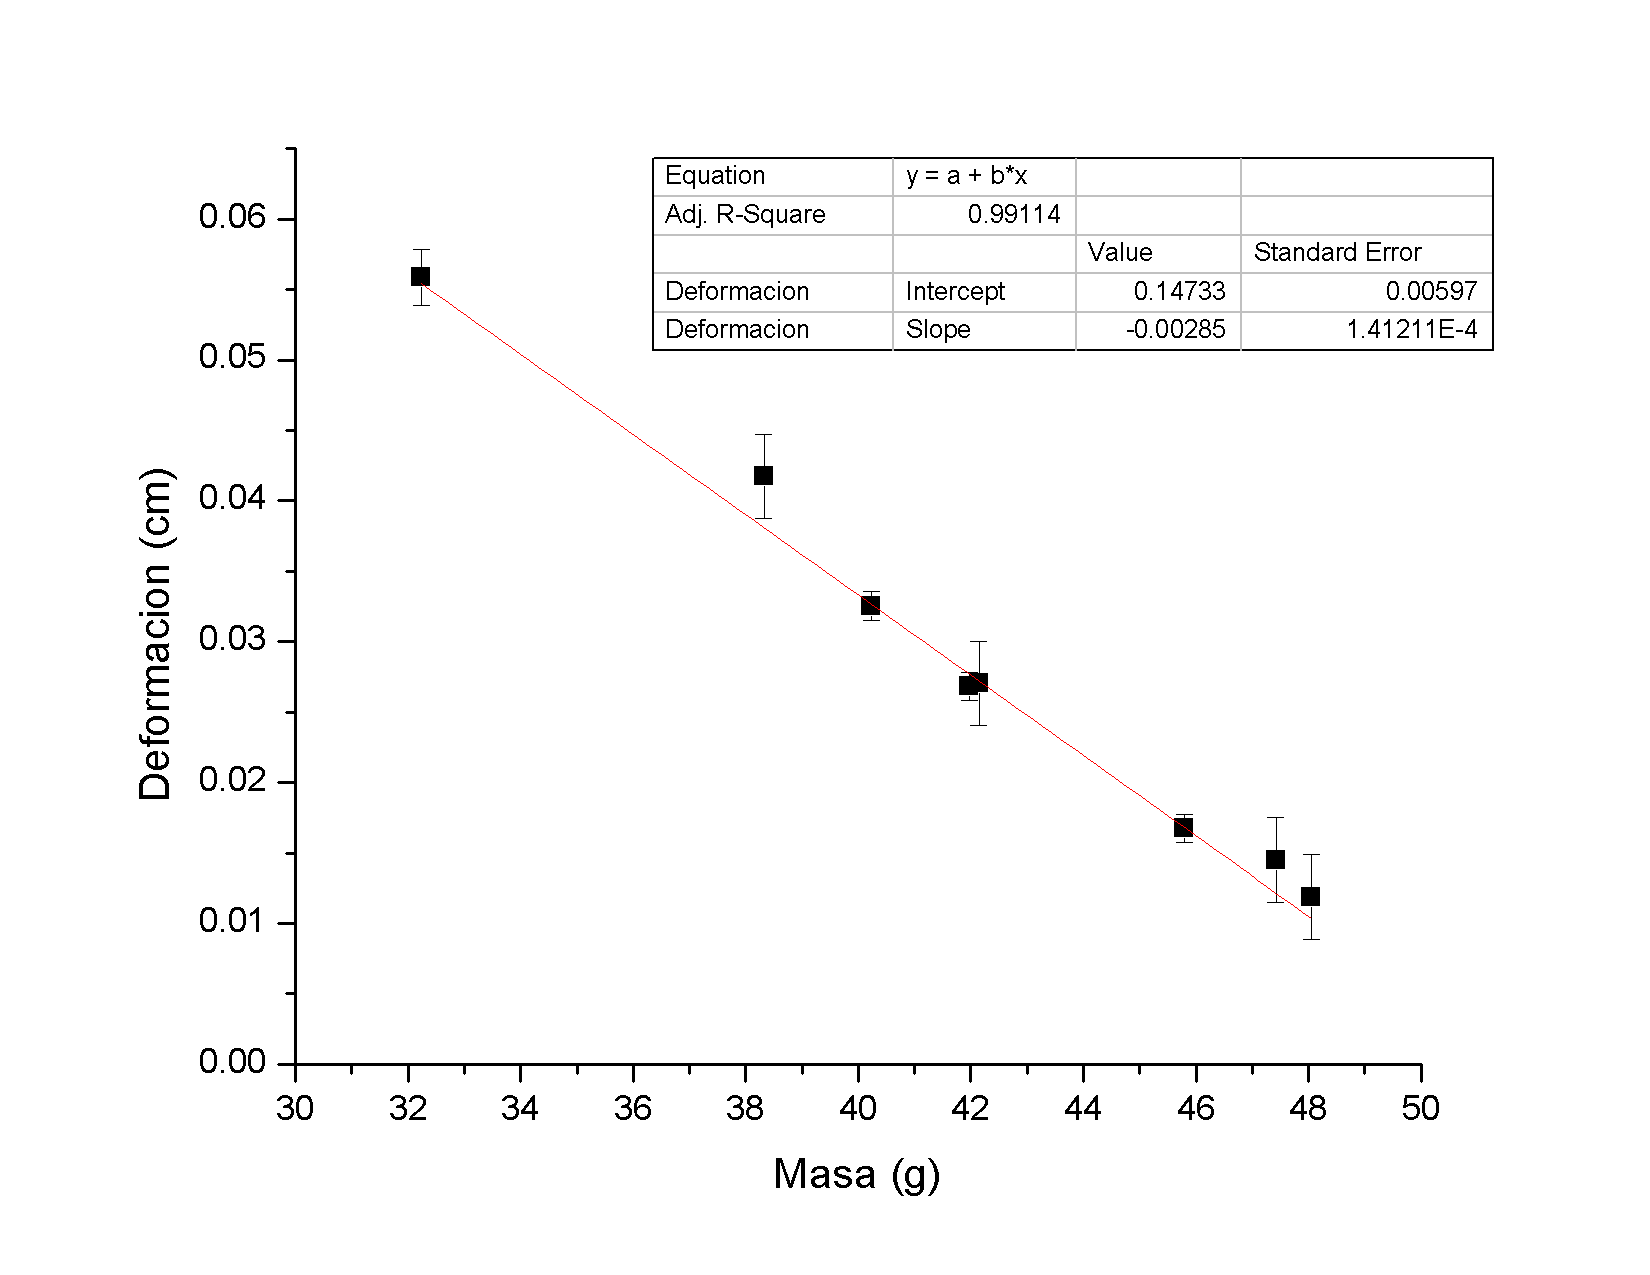
\includegraphics[width=\linewidth]{regrlin.png}
\caption{Regresi\'on lineal entre la masa y la deformaci\'on en el m\'etodo est\'atico .}
\label{fig:regrlin}
\end{figure}


\subsection{M\'etodo din\'amico}

Con los datos obtenidos de la se\~nal enviada por el fotodiodo, se realizo un ajuste exponencial sobre la misma para poder obtener el factor de amortiguamiento $\alpha$ para las tres barras, tomando como longitud total de cada barra las detalladas en la Tabla \ref{tab:valoresbarras}. \newline

En la siguiente figura, se puede observar que la se\~nal decae en el tiempo como una sinoidal con una envolvente exponencial. Tambi\'en se puede ver que se marcaron los picos de cada m\'aximo, para luego poder obtener el factor $\alpha$ mediante el ajuste mencionado al principio.

\begin{figure}[H]
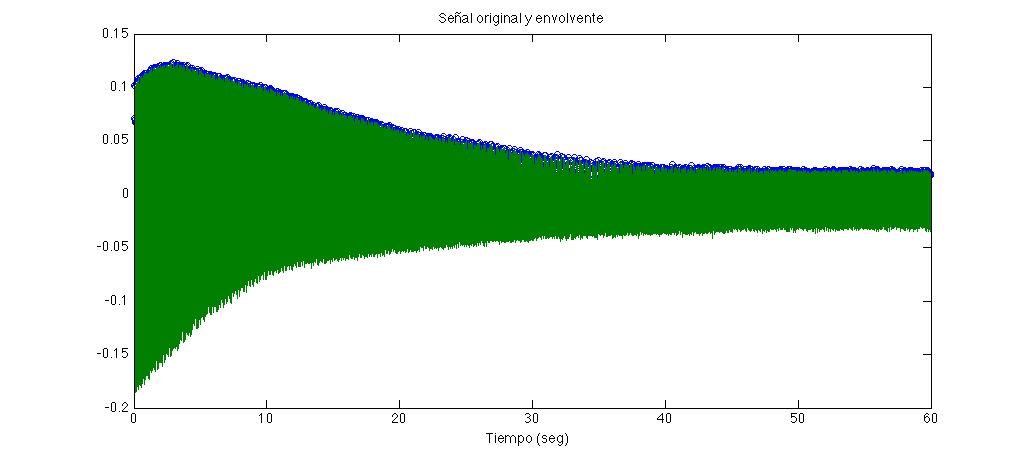
\includegraphics[width=\linewidth]{senalenvolvente.jpg}
\caption{Se\~nal obtenida para la barra de lat\'on y su envolvente.}
\label{fig:senalenvolvente}
\end{figure}

Luego, se obtuvieron las frecuencias de resonancia de cada barra mediante an\'alisis de Fourier. Como se dijo en la Introducci\'on, para la adquisici\'on de los datos se fijo un tiempo de 60 segundos y una frecuencia de sampleo de 1000 Hz. Al calcular la transformada de Fourier de la se\~nal y obtener las frecuencias, se noto que si bien aparec\'ia la fundamental y los primeros dos arm\'onicos, entre estos exist\'ian frecuencias que no correspond\'ian a modos de resonancia de la barra si no a factores tales como el efecto rebote introducido por el movimiento oscilante de la misma.

Como ejemplo, en la siguiente figura se puede ver el espectro de frecuencias de la barra de lat\'on en su longitud original $L_{1} = 31,2 \pm 0,1$ cm. Pueden apreciarse la frecuencia fundamental $f_{1} \approx 20,20$ Hz y las correspondientes al efecto de rebote ($f \approx 40,41$ Hz, etc). \newline

\begin{figure}[H]
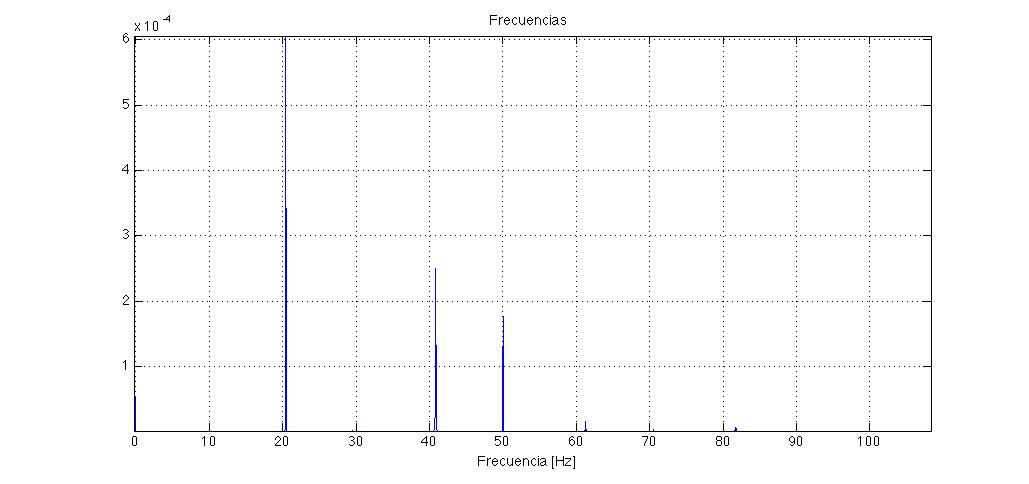
\includegraphics[width=\linewidth]{espectrolaton.jpg}
\caption{Parte del espectro de frecuencias para la barra de lat\'on. Se pueden observar la frecuencia fundamental $f_{1} \approx 20,2$ Hz y frecuencias del rebote.}
\label{fig:espectrolaton}
\end{figure}

Si bien para calcular el m\'odulo de Young solo se utiliz\'o la frecuencia del modo fundamental (y su correspondiente $k$), se pudo obtener las frecuencias del primer y segundo arm\'onico. Esto resulto mas dif\'icil de observar en los espectros debido a que los picos correspondientes a estas frecuencias era muy peque\~nos con respecto al del fundamental.\newline Siguiendo con el ejemplo de la barra de lat\'on, se calcularon dichas frecuencias mediante la ecuacion (\ref{eq:omegas}) junto con la constante de amortiguamiento $\alpha$, obteniendo los siguientes valores: $f_{1} \approx 20,20$ Hz, $f_{2} \approx 122,50$ Hz y $f_{3} \approx 354$ Hz. \newline

\begin{figure}[H]
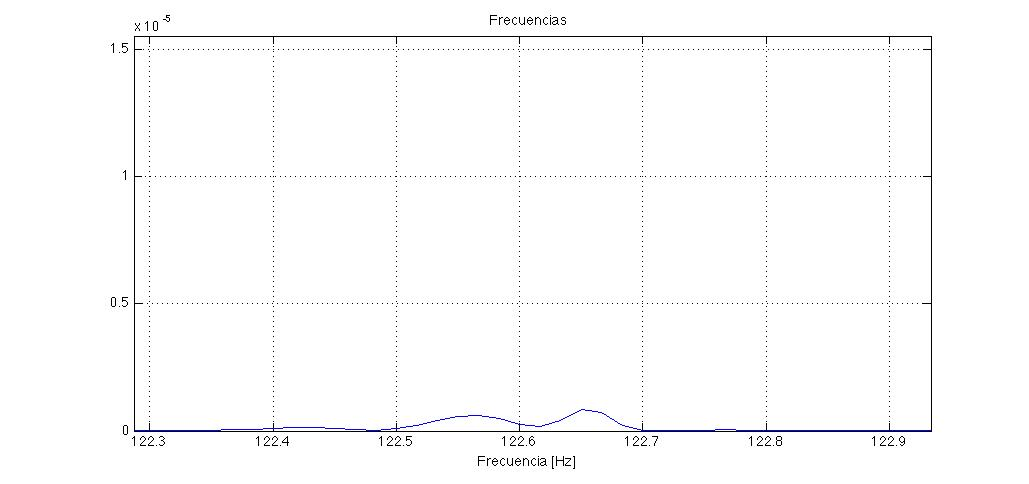
\includegraphics[width=\linewidth]{espectrolatonarmonico.jpg}
\caption{Parte del espectro de frecuencias para la barra de lat\'on. Al aumentar el zoom en el espectro, se puede observar el primer arm\'onico con frecuencia $f_{2} \approx 122,50$ Hz, con una amplitud muy peque\~na en relaci\'on a $f_{1} \approx 20,20$ Hz}
\label{fig:espectrolatonarmonico}
\end{figure}


En la siguiente tabla se detallan los valores de la frecuencia fundamental $f_{1}$ para las tres barras, utilizando $k_{1} = \frac{1,875}{L}$ y la constante de amortiguamiento $\alpha$ correspondiente a cada una con un nivel de confianza del 95\%:


\begin{table}[H]
\centering
\caption{Frecuencias fundamentales y constantes de amortiguamiento para cada barra.}
\label{tab:fya_barras}
\begin{tabular}{|c|c|c|}
\hline
Material & $f_{1}$ (Hz) & $\alpha$ (Hz) \\ \hline
Lat\'on & 20,20 & 0,0335 $\pm$ 0,0009\\ \hline
Hierro & 21,78 & 0,1343 $\pm$ 0,0009  \\ \hline
Lat\'on fino & 8,25 & 0,0190 $\pm$ 0,0009\\ \hline
\end{tabular}
\end{table}


Adem\'as, se calcul\'o la densidad lineal de cada barra a partir de su peso y longitud, as\'i como tambi\'en el momento de inercia $I$ de acuerdo a la geometr\'ia cil\'indrica de las mismas. Estos datos se encuentran en la siguiente tabla :

\begin{table}[H]
\centering
\caption{Valores de longitud $L$, densidad lineal $\rho_{l}$ y momento de inercia $I$ para las barras de lat\'on, hierro y lat\'on fino (de arriba hacia abajo, en ese \'orden).}
\label{tab:params_barras}
\begin{tabular}{|c|c|c|}
\hline
$L$ (cm) & $\rho_{l}$ (g/cm) & $I$ $(cm^{4})$\\ \hline
31,2 $\pm$ 0,1 & 1,64 $\pm$ 0,01 & 0,0024 $\pm$ 0,0001\\ \hline
36,1 $\pm$ 0,1 & 1,01 $\pm$ 0,01 & 0,0009 $\pm$ 0,0001\\ \hline
40,3 $\pm$ 0,1 & 0,55 $\pm$ 0,01 & 0,0002 $\pm$ 0,0001\\ \hline
\end{tabular}
\end{table}


Luego, mediante la ecuaci\'on (\ref{eq:omegas}) y los datos de las Tablas \ref{tab:fya_barras} y \ref{tab:params_barras}, se obtuvieron los valores de los m\'odulos de Young de cada una de las tres barras estudiadas:

\begin{table}[H]
\centering
\caption{M\'odulo de Young $E$ de cada una de las tres barras. Se puede observar que corresponden al orden de los valores te\'oricos dados por \cite{teo:ashby}}

\label{tab:young_barras}
\begin{tabular}{|c|c|}
\hline
Material & $E$ (Pa)\\ \hline
Lat\'on & $(8,44 \pm 1,1) * 10^{10}$\\ \hline
Hierro & $(2,89 \pm 0,8) * 10^{11}$\\ \hline
Lat\'on fino & $(1,58 \pm 0,2) * 10^{11}$\\ \hline
\end{tabular}
\end{table}

Para finalizar, se analiz\'o como var\'ia la frecuencia fundamental y el factor de amortiguamiento en funci\'on de la longitud de la barra de lat\'on fino, con los par\'ametros mencionados al final de  la secci\'on 2.2

\begin{figure}[H]
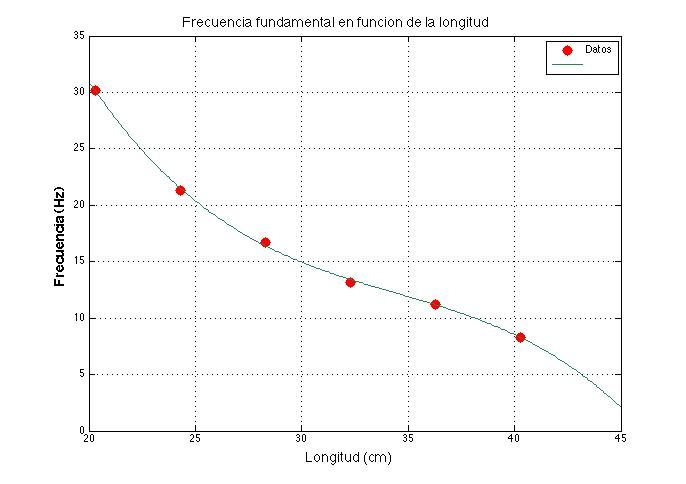
\includegraphics[width=\linewidth]{fvsl.jpg}
\caption{Frecuencias fundamentales de la barra de lat\'on fino en funci\'on de su longitud.}
\label{fig:fvsl}
\end{figure}

\begin{figure}[H]
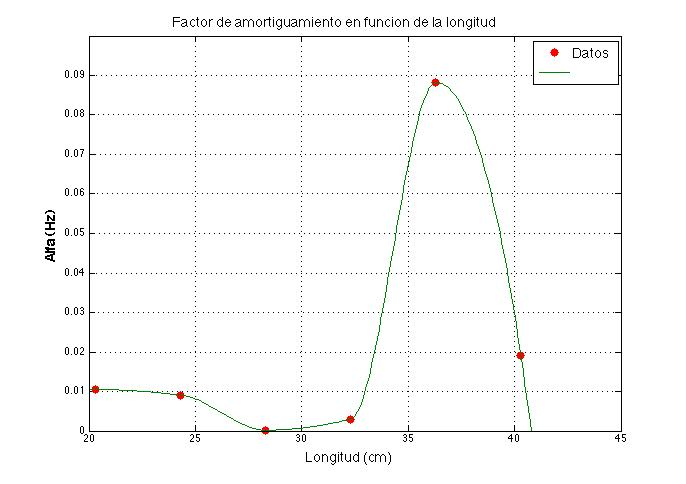
\includegraphics[width=\linewidth]{avsl.jpg}
\caption{Factor de amortiguamiento de la barra de lat\'on fino en funci\'on de su longitud.}
\label{fig:avsl}
\end{figure}

Puede apreciarse en los gr\'aficos que la frecuencia fundamental va aumentando al disminuir la longitud; dado que a menor longitud el material es mas r\'igido por lo tanto oscilar\'a a mayor frecuencia, destacando desproporcionadamente a la fundamental sobre los arm\'onicos, siendo estos \'ultimos pr\'acticamente imperceptibles en este caso. \newline

Por el contrario, si observamos el gr\'afico para el factor de amortiguamiento $\alpha$ en funci\'on de la longitud $L$; se puede destacar que para $L < L_{4} = 28,3$ cm, $\alpha$ decrece por lo tanto la barra oscilar\'a durante m\'as tiempo ocasionando que el espectro de frecuencias sea m\'as parejo, con el costo de introducir una mayor cantidad de frecuencias no deseadas.
A partir de $L > L_{4} = 28,3$ cm, $\alpha$ vuelve a crecer hasta alcanzar un valor m\'aximo en $L_{2} = 36,3$ cm. De estos valores, se pueden inferir dos comportamientos: como un sistema sobreamortiguado para $L < L_{4}$; mientras que para $L > L_{4}$ el sistema se tiende a estar amortiguado de manera cr\'itica. 

Cabe aclarar que, para esta parte de la experiencia, se intent\'o tomar longitudes m\'as cortas a $L_{6} = 20,3$ cm, pero observamos que los datos recolectados eran muy similares a una barra en reposo, por lo tanto no generaban valores significativos de $f$ y $\alpha$.

%------------------------------------------------

\section{Conclusiones}

En en el presente trabajo se calcul\'o el m\'odulo de elasticidad de Young de diferentes materiales mediante de la flexi\'on de una barra de lat\'on en voladizo. Para eso, se utilizaron dos m\'etodos: uno est\'atico y otro din\'amico. \newline

En el m\'etodo est\'atico se analizaron patrones de difracci\'on obtenidos por la luz de un laser a traves de una rendija en un extremo de una barra. Se obtuvo un valor del m\'odulo de Young que es aproximadamente el doble de los valores tabulados en la literatura y de los que obtuvimos mediante el m\'etodo din\'amico, sin embargo son del mismo orden de magnitud. \newline

Se considera que al ser un m\'todo indirecto, pasando tanto por un m\'etodo \'optico como por varias mediciones directas, los errores tienden a propagarse. Por otro lado, tambi\'en concluimos que esta diferencia entre el valor obtenido y el tabulado puede ser producido por un mal ajuste del tornillo sujetador de la varilla, pues este sujetador consist\'ia en dos tornillos en diferentes posiciones de los cuales uno no ajustaba completamente. \newline


En el m\'etodo din\'amico, se obtuvieron las frecuencias de oscilaci\'on y la constante de amortiguamiento de tres barras: dos de lat\'on (diferenciandose en su diametro y longitud) y otra de hierro. 

Con los datos obtenidos, se realizo un ajuste para poder obtener el factor de amortiguamiento $\alpha$ para las tres barras, tomando como longitud total de cada barra las expuestas en la Tabla \ref{tab:params_barras}.

Luego, se obtuvieron las frecuencias de resonancia realizando una transformada de Fourier a la se\~nal original. Pudimos ver a frecuencia fundamental y los primeros arm\'onicos, no obstante entre estos exist\'ian frecuencias que no correspond\'ian a modos de resonancia de la barra si no a diversos factores como un efecto rebote introducido por el movimiento oscilante de la misma registrado por el fotodiodo. \newline

En la pr\'actica, para calcular el m\'odulo de Young solo se utiliz\'o la frecuencia del modo fundamental; como se menciono en el p\'arrafo anterior, logramos obtener las frecuencias del primer y segundo arm\'onico, las cuales resultaron dif\'iciles de visualizar dado que los picos correspondientes a estas frecuencias eran muy peque\~nos con respecto al del fundamental. Cabe destacar que, con este m\'etodo se logro una medici\'on mucho m\'as precisa que con el m\'etodo est\'atico; si bien ambas mediciones dan en el orden de $10^{10}$, el valor de $E$ calculado es muy similar a los encontrados en la bibliograf\'ia para el material considerado.\newline

Por \'ultimo, se estudi\'o la variaci\'on de la frecuencia fundamental y el factor de amortiguamiento en funci\'on de la longitud para la barra de lat\'on fino, con lo cual concluimos que
la frecuencia fundamental aumenta al disminuir la longitud de manera exponencial; esto puede deberse a que, a menor longitud, el material adquiere m\'as r\'igidez, por lo tanto oscila a frecuencias m\'as altas, destacando a la fundamental sobre sus arm\'onicos, siendo \'estos \'ultimos muy dif\'iciles de ver en los espectros. \newline

Por otro lado, al observar el factor de amortiguamiento $\alpha$ en funci\'on de la longitud se pudo observar que decrec\'ia para los valores mas bajos de longitud; luego se llegaba a un valor de $\alpha$ m\'inimo (en nuestro caso el correspondiente a $L_{4} = 28,3$ cm) para volver a crecer y alcanzar un m\'aximo en $L_{2} = 36,3$ cm. Puede concluirse que este sistema se comporta como un sistema sobreamortiguado para $L < L_{4}$; mientras que para la regi\'on $L > L_{4}$ es comparable con un sistema con amortiguamiento cr\'itico. 

%----------------------------------------------------------------------------------------
%	REFERENCE LIST
%----------------------------------------------------------------------------------------
\newpage
\begin{thebibliography}{99} % Bibliography - this is intentionally simple in this template


\bibitem{eq:leyhooke} M. Alonso, E. J. Finn, \textit{F\'isica - Vol. 1}, Editorial Addison-Wesley Iberoamericana (1986), p\'ag. 363

\bibitem{eq:vigas} W. Seto, \textit{Theory and problems of mechanical vibrations}, Editorial McGraw Hill, 2da edici\'on, Barcelona (1971), Cap. 9
\bibitem{eq:vigadyns} S. C. Hunter, \textit{Mechanics of continuous media}, John Wiley and Sons (1986)
\bibitem{teo:shannon} S. Ghosh, \textit{Signals and Systems}, Editorial Pearson Education, India (2006), Cap. 3
\bibitem{teo:ashby} M. F. Ashby, D. R. H. Jones, \textit{Materiales para Ingenier\'ia 1 - Introducci\'on a las propiedades, las aplicaciones y el dise\~no}, Editorial Revert\'e S.A., edici\'on en espa\~nol, Barcelona (2008), p\'ag. 39

 
\end{thebibliography}


%----------------------------------------------------------------------------------------

\end{document}